\documentclass{article}
\usepackage{importer}

\usepackage[backend=biber]{biblatex}
\addbibresource{kilder.bib}

\title{Forelesningsnotater: Faste Stoffers Fysikk}
\author{Sebastian Siljuholtet Johansen }
\date{Vår 2024}

\begin{document}

\maketitle

\newpage
\section*{Ingress}
Skrevet av studenter. Notater er tatt under forelesningene i TFY4220 Faste Stoffers Fysikk av Dag Werner Breiby. I tillegg har visse deler blitt utdypet og ekstra forklaringer har blitt lagt til visse deler.
\newpage
\tableofcontents

\newpage
\section{Kapittel I: }
Hvordan atomer er ordnet kalles for \enquote{struktur}. Denne strukturen bestemmer egneskapene til et materiale. Altså hvordan det oppfører seg.

Vi diskuterer to slike typer av krystallinske materialer:
\begin{itemize}
    \item Amorfisk (glass, væsker, ...): som betyr tilfeldig.
    \item Krystallinske: som betyr periodisk i rom (i realiteten finnes det defekter).
\end{itemize}
Av disse krystallinske materialene har vi to typer:
\begin{itemize}
    \item Enkeltkrystaller: Som betyr at de har en uniform struktur.
    \item Polykrystaller: Disse er bygd opp av flere ulike periodiske strukturer i et materiale. På en måte en slags kobling av flere enkeltkrystaller. Hver enkelt av disse delene kalles for ulike korn. 
\end{itemize}
En tegning av disse er:
\begin{figure}
    \centering
    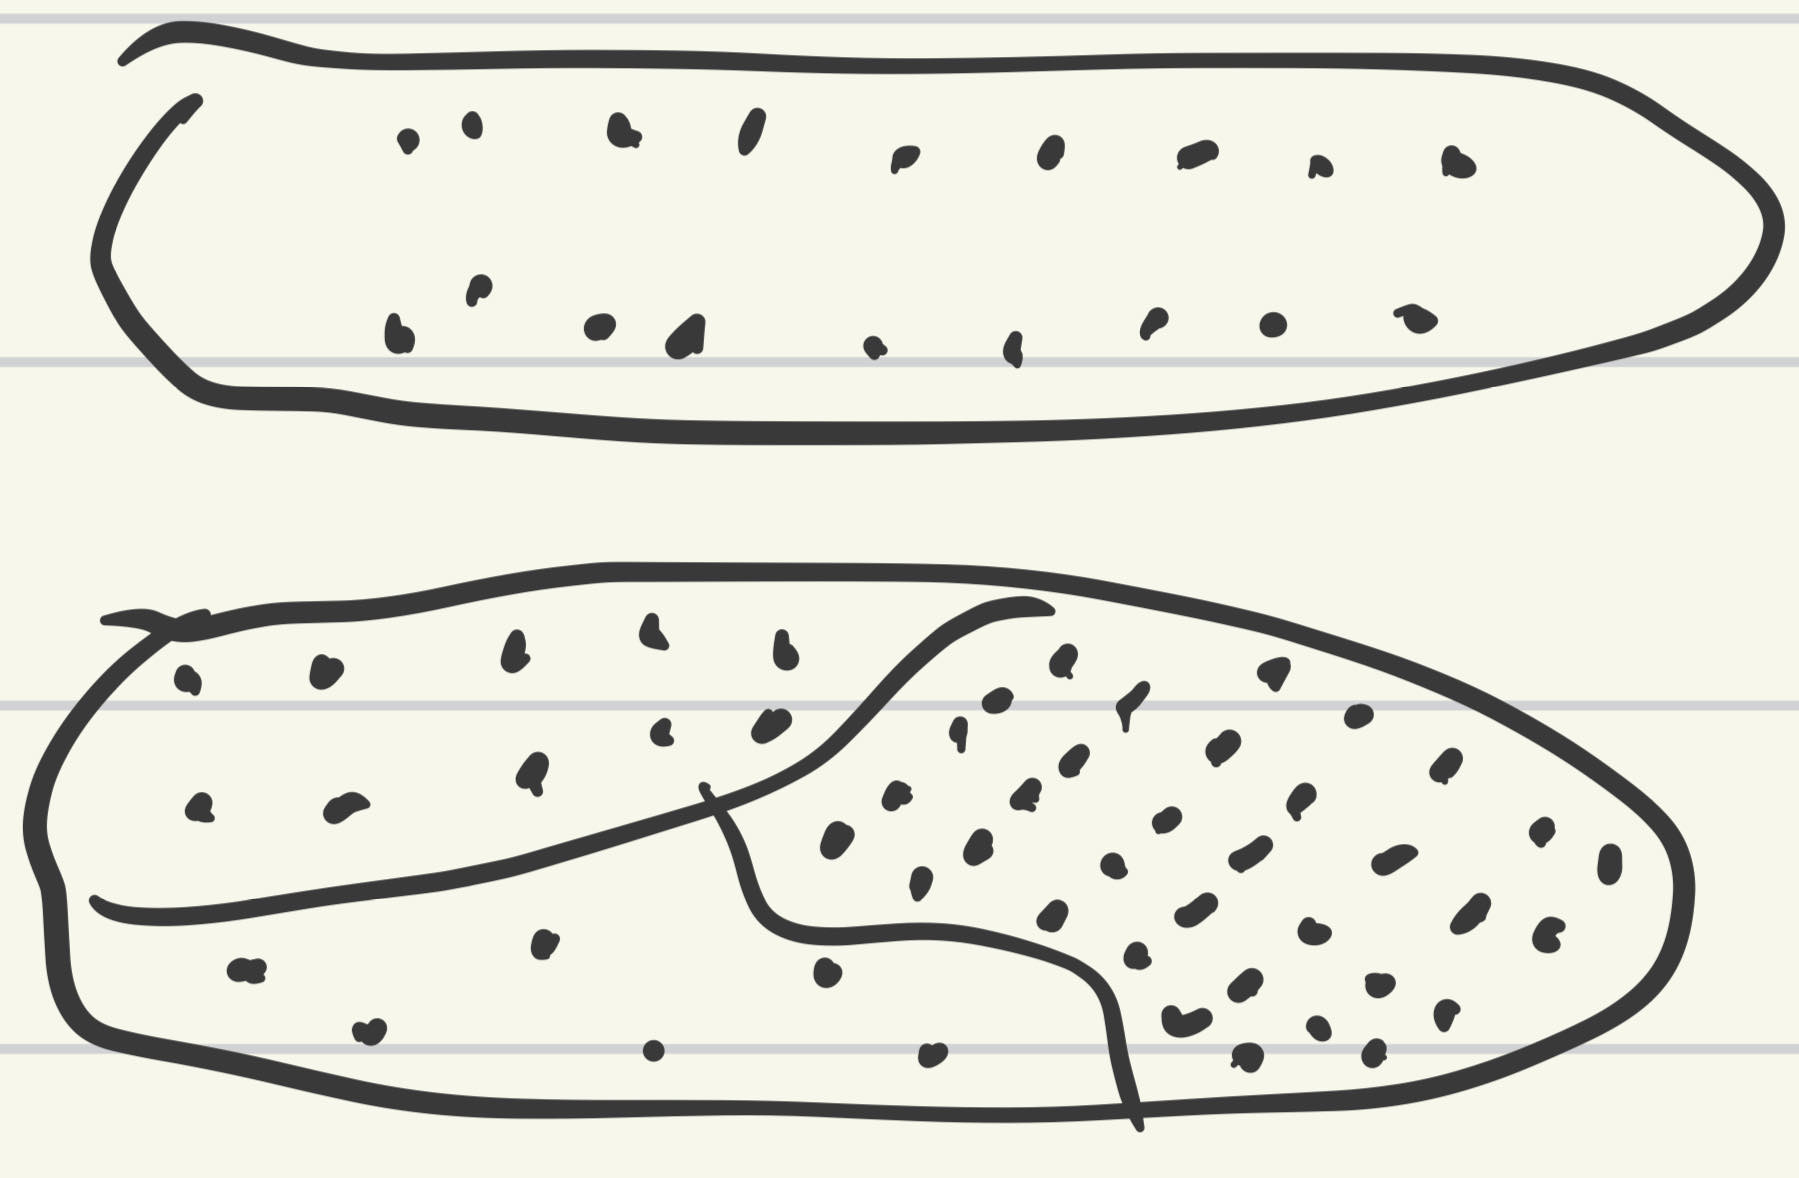
\includegraphics[width=0.5\linewidth]{bilder/enkelt_poly_krystaller.png}
    \caption{Enkelt krystall(over) og poly-krystall(under)}
    \label{fig:enkelt_poly_krystaller}
\end{figure}
I disse enkeltkrystallene har vi en eller annen translasjonell symmetri i domenet deres. Slik som en rotasjon, en speiling eller rene translasjoner.
\subsection{Bravais Gitter}
Et slikt gitter er bygd opp av en uendelig mengde med punkter som ser likt ut fra hvert eneste punkt. I en viss dimensjon d kan vi definere ethvert slikt punkt som:
\begin{align*}
    \vec{R} = \sum_{i} n_i \vec{a}_i
\end{align*}
I 2 dimensjoner finnes det kun 5 gyldige Bravais-gittere som alle er repeterende versjoner av 5 ulike figurer. Disse er repeterende firkant-, rektangulært-, heksagonalt-, sentrert-rektangulært og skråmønstere. Videre finnes det i 3 dimensjoner:
\begin{itemize}
    \item Triklinisk: $a\ne b\ne c$, $\alpha \ne \beta \ne \gamma \ne 90$ = 3D prisme
    \item Monoklinisk: $a \ne b \ne c$, $\beta \ne 90$, $\alpha = \gamma = 90$
    \item Ortorombisk: $a \ne b \ne c$, $\alpha = \beta = \gamma = 90$
    \item Tetragonalt: $a = b \ne c$, $\alpha = \beta = \gamma = 90$
    \item Kubisk: $a = b = c$, $\alpha = \beta = \gamma$. Dette er det vi vil se på.
\end{itemize}
Totalt finnes det 14 stykker av disse.
\subsubsection{Kubiske systemer}
Det finnes flere forskjellige kubiske systemer. Det er tre stykker vi ser på her. Disse kan tegnes som under \cite{kubiske_systemer}:
\begin{figure}[h!]
  \centering
  \begin{subfigure}{0.3\textwidth}
    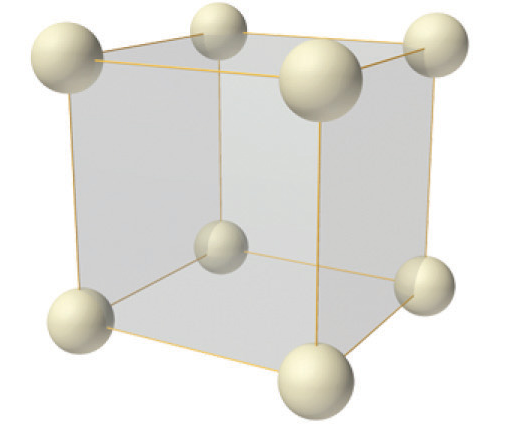
\includegraphics[width=\linewidth]{bilder/enkelt_kubisk.png}
    \caption{Enkelt kubisk}
    \label{fig:enkelt_kubisk}
  \end{subfigure}
  \begin{subfigure}{0.3\textwidth}
    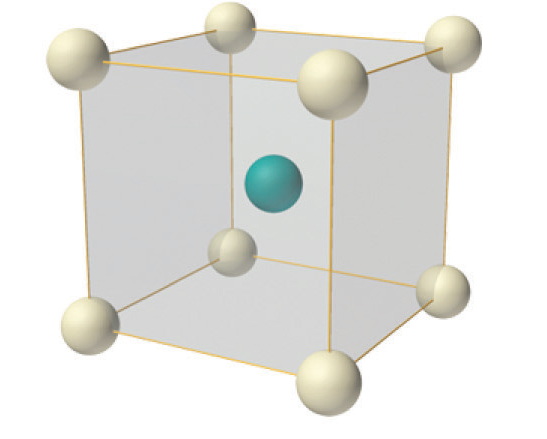
\includegraphics[width=\linewidth]{bilder/romsentert_kubisk.png}
    \caption{Romsentrert kubisk}
    \label{fig:romsentert_kubisk}
  \end{subfigure}
  \begin{subfigure}{0.3\textwidth}
    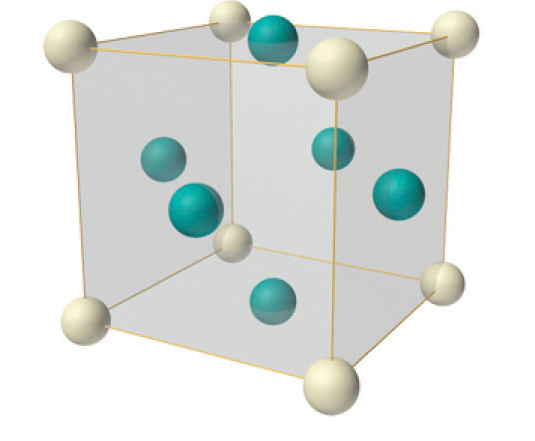
\includegraphics[width=\linewidth]{bilder/flatesentrert_kubisk.png}
    \caption{Flatesentrert kubisk}
    \label{fig:flatesentrert_kubisk}
  \end{subfigure}
  \caption{Forskjellige typer kubiske systemer}
  \label{fig:kubiske_interpolasjoner}
\end{figure}
\newpage
\section{Kapittel II: }
\newpage
\section{Kapittel III: }
\newpage
\section{Kapittel IV: }
\newpage
\section{Kapittel V: }
\newpage
\section{Kapittel VI: }
\newpage
\section{Kapittel VII: Energibånd }
% Forelesning {13.03.2024 10:15-12:00}
\subsection{Blocks Teorem}
\subsubsection{Oppsummering av Sentrallikningen}
Så langt har vi funnet at for frie elektroner så følger de følgende energirelasjon:
\begin{equation}
  \label{eq:energi_for_frie_elektroner}
  E_k = \frac{\hbar^2 k^2}{2m}
\end{equation}
Hvis vi plotter denne ser den ut som en parabol. Vi har funnet ut at i våre periodiske potensialer så kan vi finne energibåndgap, altså hakk i denne parabolen. Da bånd fra en y til en annen y, hvor vi ikke finner noen energier. Altså har vi ulovlige energibånd. Dette skaper ulike egenskaper i materialer % legg til mer info.

For et periodisk potensial fant vi at vi fikk Bragg spredning av elektronbølger. Videre fant vi også ståebnde bølger i krystaller.

Vi fant også \underline{Block-Funksjonene}. Disse så generelt slik ut:
\begin{equation}
  \label{eq:block_funksjoner}
  \psi_{\vec{k}}(\vec{r}) = e^{i\vec{k}\cdot\vec{r}}u_k(\vec{r})
\end{equation}
Disse var da løsningene til Schrödingerlikningen med et periodisk potensial.
Videre ser Schrödinger likningen slik ut for et potensial:
\begin{align}
  \label{eq:schrödinger_likningen_med_periodisk_potensial}
  \left\{  -\frac{\hbar^2}{2m}\nabla^2 + u(\vec{r})  \right\}\psi(\vec{r}) = E\psi(\vec{r}) \\
  u(\vec{r}) = u(\vec{r} + \vec{R})
\end{align}
Altså blir potensialet her $\vec{R}$-periodisk. Ved å nå bruke foriertransformer så kan vi gjøre om denne differensiallikningen til en algebraisk likning. fouriertransformene er definert slik:
\begin{align*}
  \psi(x) &= \sum_k c_k e^{ikx} \\
  u(x) &= \sum_G u_g e^{iGx}
\end{align*}
Disse gir oss "sentralelikningen":
\begin{equation}
  \label{eq:den_sentrale_likningen}
  \left(\frac{\hbar^2 k^2}{2m} - E\right)c_k + \sum_G u_g c_{k-G} = 0
\end{equation}
Denne likningen kobler hver ukjente koeffisient $c_k$ til et lite underset av alle andre $c_k$. Dette ser vi fra at $k$ er definert fra periodiske grensebetingelser som gir oss at $k = \frac{2\pi}{L}$, mens g er definert ut i fra krystallgitteret vårt. Altså: $G = \frac{2pi}{a}$. Siden $a >> L$ så blir stegene mellom $G$-ene enormt mye større enn de mellom $k$-ene. Da ser vi at vi har veldig mange flere $k$-er for hver $g$. Dermed kobles bare hver $c_k$ til et lite undersett av alle $k$-ene. Her blir da $G$-rommet et underrom av $k$-rommet.

Mer mattematisk så kobler for eksempel $c_{k_0}$ til $\{..., c_{k_0 - 2g}, c_{k_0 - g}, c_{k_0}, c_{k_0 + g}, c_{k_0 + 2g}\}$

\subsubsection{Å Bevise Teoremet}
La oss nå anta at vi har en løsning til bølgefunksjonen $\psi(\vec{r})$.
Her kan vi da gjøre:
\begin{align*}
  \psi(\vec{r}) &= \sum_{\vec{k}} c_{\vec{k}} e^{i \vec{k} {r}} \\
  \text{Gjennom sentrallikningen får vi:} \\
   \psi_k(\vec{r})&= \sum_{\vec{G}} c_{\vec{k} - \vec{G}} e^{i(\vec{k} - \vec{G}) 
   \vec{r}} \\
   &= e^{i\vec{k}\cdot\vec{r}} \sum_{\vec{G}}  c_{\vec{k} - \vec{G}}e^{-i \vec{G}\cdot\vec{R}}
\end{align*}
Summen over $\vec{G}$ til slutt kan vi se at er $\vec{R}$ periodisk. Altså kunne vi ha kalt hele summen for en funksjon som er periodisk. Ved å sammenligne med definisjonen av Block-funksjonene, så har vi faktisk bevist at de er gyldige løsninger. Vi trenger bare å kalle summen for for $u(\vec{r})$ som vi brukte i definisjonen deres: 

\begin{equation*}
  u_k(\vec{r}) = \sum_{\vec{G}} c_{\vec{k} - \vec{G}} e^{-i \vec{G} \cdot \vec{R}}
\end{equation*}
\subsubsection{Konsekvensene til Block's teorem}
Vi antar at vi har $\psi_{k'}(\vec{r})$ for en gitt $\vec{k'}$. Da kan vi skrive fra Block's teorem, at: $\psi_{k'}(\vec{r}) = e^{i\vec{k}\cdot\vec{r}} u_{k'}(\vec{r})$. Nå lar vi: $\vec{k} = \vec{k'} + \vec{G}$, hvor $\vec{G}$ er en resiprokalgittervektor. Nå kan vi da skrive:
\begin{align*}
  \psi_k{\vec{r}} &= e^{i \vec{k} \cdot \vec{r}} e^{i \vec{G} \cdot \vec{r} u_{\vec{k} - \vec{G}}u(\vec{r})} \\
  &= e^{i\vec{k}\cdot\vec{r}}{u'}_{\vec{k}-\vec{g}}
\end{align*}
Hvor: ${u'}_{\vec{k}-\vec{g}} = {u}_{\vec{k}-\vec{g}} e^{-i \vec{G}\cdot \vec{r}}$.
Denne nye Blockfunksjonen er \underline{like god} på alle måter som den originale. Konsekvensen her er at bølgevektoren $\vec{k}$ er vilkårlig med hensyn til addisjonen av en resiprokalgittervektor.

\subsection{Fyllingen av Elektronbåndene}
Fra de periodiske grensebetingelsene så får vi at: $\Delta k = \frac{2\pi}{L} = \frac{2\pi}{Na}$. Hvis vi nå sier at $\vec{k}$-verdiene innenfor  Brillouin-sonen (enhetscellen i k-rommet) $\left[-\frac{\pi}{a}, \frac{\pi}{a} \right]$, skaper et bånd, så ser vi at hvert bånd har N mulige k-verdier. Men hver av disse verdiene kan enten ha spin opp ($\uparrow$) eller ned ($\downarrow$). Altså har vi N tilstander per slikt bånd, med totalt 2N elektroner.

Hvis vi har \underline{et} valenselektron i hver primitive enhetscelle så vil materialet vårt være et \underline{metall}. Hvis det er \underline{to} valenselektroner per primitive enhetscelle så kan et bånd være helt fyllt, men ikke nødvendigvis. I 3 dimensjoner så kan båndene krysse over hverandre. Ved at disse båndene krysser hverandre mener jeg at: % fyll inn mer her.

\subsubsection{Tomgitter Tilnærming}
I denne tilnærmingen lar vi potensialet $u \rightarrow 0$. Da blir alle Fourier-koeffisientene $u_g \rightarrow 0$. Konsekvensen her blir klart da at båndgapene forsvinner. Da blir sentrallikningen forenklet til at vi får frie elektroner igjen, som forventet. Det som er spennende å se på i denne frie modellen er hvordadan vi får energibånd får hver eneste $\vec{G}$. Dette er fordi alle løsninger med $\vec{k}$ vil også skape løsningene $\vec{k} + n \vec{G}, \tab[0.5cm] \vec{G} \in \mathbb{Z}$ Altså vil vi få veldig mange energinivåer: $E_n(\vec{k}) = \frac{\hbar^2(\vec{k} + \vec{G}_n)^2}{2m}$. Dette kan vi i se i bildet under:
\begin{figure}[h]
  \centering
  \caption{1D - Overlappende Tomgitter Tilnærming: \cite{WikipediaEN:Empty_lattice_approximation}}
  \includegraphics[scale=0.1]{bilder/1d_overlappende_tomgitter_tilnærming.png}
  \label{fig:1d_overlappende_tomgitter_tilnærming}
\end{figure}
%Forelesning 03.04.2024
\subsubsection{Litt høyre potensial(fortsatt svakt)}

Fra kapittel 6 fant vi en dispersasjonsrelasjon for frie elektroner: $E = \frac{\hbar^2 k^2}{2m}$. I denne modellen så er alle materialer metaller siden vi alltid har et nytt nivå vi kan dytte elektroner opp i så de kan bevege seg "fritt". I kapittel 7 introduserte vi Bloch-funksjoner og fant ulike energibånd.
 I tillegg deriverte vi sentrallikningen: $\left(\frac{\hbar^2 k^2}{2m} - E\right) c_K + \sum_G u_G c_{k - G} = 0$. 

Videre så vi at i grensen $u_G \rightarrow 0$ så kunne disse parabolene overlappe slik som i figuren over i tomgittertilnærmingen \ref{fig:1d_overlappende_tomgitter_tilnærming}.

La oss nå øke potensialet (forstatt svakt) og anta at: $u(x) = 2 u_g cos(\frac{2\pi x}{G}) = \sum_G u_G e^{iGx}$, hvor $u_G$ er reell. Vi har også at $u_G = u_{-G}$ fra tidligere. Vi definerer nå at $u_g = u_{-g} = u$ hvor alle andre $u_G=0$. La oss nå se på sentrallikningen:
\begin{align*}
  \left(\frac{\hbar^2 k^2}{2m} - E \right)c_k &+ \sum_G u_G c_{k-G} = 0 \\
  \left(\frac{\hbar^2 k^2}{2m} - E \right)c_k  &+ ... \\
  &+ u_{-2g} c_{k - (-2g)} \\
  &+ u_{-g} c_{k - (-g)} \\
  &+ u_{0} c_{k} \\
  &+ u_{g} c_{k - g} \\
  &+ u_{2g} c_{k - 2g}  = 0\\
\end{align*}
Her kan vi simplifisere dette utrykket siden alt annet enn $u_g$ og $u_{-g}$ blir lik null siden vi antok det før vi begynte. Altså får vi:
\begin{align*}
  \left(\frac{\hbar^2 k^2}{2m} - E \right)c_k  &+ ... \\
  &+ u_{-2g} c_{k - (-2g)} \\
  &+ u_{-g} c_{k - (-g)} \\
  &+ u_{0} c_{k} \\
  &+ u_{g} c_{k - g} \\
  &+ u_{2g} c_{k - 2g}  = 0 = \\
  \left(\frac{\hbar^2 k^2}{2m} - E \right)c_k  &+ ... \\
  &+ u_{-g} c_{k - (-g)} \\
  &+ u_{g} c_{k - g} = 0
\end{align*}
Men nå vet vi jo at $k\rightarrow k-g$ også er en løsning. Altså gjelder også:
\begin{align*}
  \left(\frac{\hbar^2 k^2}{2m} - E \right)c_k  &+ ... \\
  &+ u_{-g} c_{k - g - (-g)} \\
  &+ u_{g} c_{k - g - g} = 0
\end{align*}
Videre så er jo også $k \rightarrow k+g$ og $k\rightarrow k+2g$ og så videre for evig. Vi kan få dette i matriseform. Vi skriver derfor at: $\lambda_k \defeq \frac{\hbar^2k^2}{2m}$ og får:
\begin{align*}
  \begin{bmatrix}
    \lambda_{k-2g} - E& u_g & 0 & 0 & 0 \\
    u_g & \lambda_{k-g} - E & u_g & 0 & 0\\
   0 & u_g & \lambda_{k} - E &  u_g  & 0 \\
   0& 0 & u_g & \lambda_{k+g} - E& u_g  \\
   0& 0 & 0 & u_g & \lambda_{k+2g} - E  \\
  \end{bmatrix} \begin{bmatrix}
  c_{k-2g} \\
  c_{k - g} \\
  c_{k} \\
  c_{k+g}\\
  c_{k+2g}
  \end{bmatrix} = 0 \\
\Rightarrow \left | \begin{bmatrix}
    \lambda_{k-2g} - E& u_g & 0 & 0 & 0 \\
    u_g & \lambda_{k-g} - E & u_g & 0 & 0\\
   0 & u_g & \lambda_{k} - E &  u_g  & 0 \\
   0& 0 & u_g & \lambda_{k+g} - E& u_g  \\
   0& 0 & 0 & u_g & \lambda_{k+2g} - E  \\
  \end{bmatrix} \right | = 0
\end{align*}
Vi kan trekke ut en mindre determinant av denne med dominante termer. Vi velger firkanten 11-22:
\begin{align*}
  \left | \begin{bmatrix}
      u_g & \lambda_{k-g} - E & u_g\\
     u_g & \lambda_{k} - E &  u_g \\
    \end{bmatrix} \right | &= 0 \\
     \Rightarrow (\lambda_{k-g} - E)(\lambda_k - E) - u_g^2 &= 0 \\
     \Rightarrow E(k) &= \frac{1}{2}\left(\lambda_k + \lambda_{k-g}\right) \pm \left[\frac{1}{4}\left(\lambda_{k-g} - \lambda_k\right) +u_g^2 \right]^{\frac{1}{2}}
\end{align*}

Ved å nå ta for oss sone-grensen $k=\frac{g}{2} = \frac{\pi}{a}$ så får vi at:
\begin{align*}
  \lambda_k &= \frac{\hbar^2 k^2}{2m} = \frac{\hbar^2}{2m}\frac{g^2}{4} \\
  \lambda_{k-g} &= \frac{\hbar^2(k-g)^2}{2m} = \frac{\hbar^2 (\frac{g}{2}-g)^2}{2m} = \lambda_k \\
  \Rightarrow E(B.Z) = E\left(\frac{g}{2}\right) &= \lambda_{\frac{g}{2}} \pm u_g = \frac{\hbar^2 (\frac{1}{2}g)^2}{2m} \pm u_{1} = \underbrace{\frac{\hbar^2 \left(\frac{\pi}{a}\right)^2}{2m}}_{\text{Fritt elektron } E = \frac{\hbar^2 k^2}{2m}} \pm \underbrace{u_{1}}_{\text{Båndgap av størrelse } 2u_1}
\end{align*}

Vi kan oogså vise at: 

A: $\psi_{k = \frac{g}{2}}(x) = e^{i g \frac{x}{2}} \pm e^{-ig\frac{x}{2}}$, som er en stående bølge. Se kapittel 7

B: $u_g = 0$, på grensen til B.Z-en

C: Nær nok grensen til B.Z-en så er båndstrukturen parabolsk.

\subsubsection{Parabolske bånd}
For et fritt elektron hadde vi jo da: $E = \frac{\hbar^2 k^2}{2m}$, som er parabolsk, men hvordan gjør vi de andre elektronene parabolske også? Vel vi vil introdusere en effektiv masse $m^*$. Men hvorfor ville massen ha endret seg? Den vil endre seg fordi elektronet vil vekselvirke med omgivelsene (ionene rundt seg), og dermed vil bevegelsen dens være vanskeligere å idusere. Altså øker "treghetsmomentet" dens og dermed "massen" og den effektive massen.
\subsubsubsection{Krystall momentum}
$\vec{k}$ kan enten bli tolket som en bølgevektor eller som 3 kvantetall. $\hbar\vec{k}$ er \underline{ikke} det reelle/fysiske momentumet til elektronene. Vi har at $\hat{p} = -i \hbar \nabla$. For en Bloch-tilstand: $\psi_k(\vec{r}) = e^{i \vec{k} \cdot \vec{r}} u_k(\vec{r})$. La oss nå bruke $\hat{p}$ på denne:
\begin{align*}
  \hat{p} \psi_k(\vec{r}) = -i \hbar \nabla \psi_k(\vec{r}) = \underbrace{\hbar \vec{k} \psi_K (\vec{r}) - e^{i \vec{k} \cdot \vec{r}} i \hbar \nabla u_k(\vec{r})}_{\text{Ingen skarp egenverdi}}
\end{align*}
Selv om vi ikke har noen skarp egenverdi så er $\hbar \vec{k}$ fortsatt nyttig. Det er kalt krystall-momentum.
\subsubsubsection{Gruppehastighet og effektiv masse}
Vi husker at gruppehastighet er definert som: $v_g = \frac{d \omega(k)}{dk} = \frac{1}{\hbar} \frac{dE(k)}{dk}$.

Som gir oss aksellerasjonen: $a = \frac{d v_g}{dt} = \frac{1}{\hbar} \frac{d}{dt} \frac{dE(k)}{dk} = \frac{1}{\hbar}\left (\frac{d^2 E(k)}{dk^2} \frac{dk}{dt}\right)$.

Hvis vi nå ser på et eksternt felt fra newtons lov: $\hbar \frac{dk}{dt} = -e \varepsilon$

Som fører til at: $a = -\frac{1}{\hbar^2} \frac{d^2 E}{dk^2} e \varepsilon$.

Hvis vi nå definerer at $m^* = \left(\hbar^2 \frac{d^2 E}{dk^2}\right)^{-1}$ så får vi at $m^*a=-e\varepsilon$.

For frie elektroner blir jo da $m^* = m$, fra: $\frac{d^2 E}{dk^2} = \frac{d^2}{dk^2} \left(\frac{\hbar^2 k^2}{2m}\right) = \frac{\hbar^2}{m}$

%Forelesning 08.04.2024
\newpage
\section{Kapittel VIII: Halvledere}
Ved null temperatur vil halvledere bli til insulatorer. Dette er fordi ved null temperatur vil et system ha falt ned i alle orbitalene så alle elektronene "sitter fast". Altså kreves det mye energi og et stort potensial over stoffet for å få til at elektroner hopper ut av disse orbitalene og begynner å bevege seg. 
Altså kan vi si for halvledere at:
\begin{itemize}
  \item Konduktivitet øker når temperatur øker. Dette blir da fordi fler elektroner eksiteres til ledningsbåndene eller nærmere dem ved en høyere temperatur. Da er det lettere å bevege dem og dermed har vi som sagt at konduktiviteten øker.
  
  NB!: I metaller vil en økende temperatur føre til mer og mer fononvekselsvirkninger som forstyrrer elektronene og dermed minker konduktiviteten.
  \item De har et båndgap på $\le 3 \text{eV}$.
  \item De har en ladningsbærerkonsentrasjon som er mye lavere enn for metaller. Altså har vi for metaller at $n \propto 10^{23} \ cm^{-3}$ elektroner, mens vi har opp til $n \propto 10^{13} \ cm^{-3}$ for halvlederen Germanium ved romtemperatur. Grunnen til at jeg spesifiserer romptemperatur er fordi metallene vil være fyllt opp med elektroner, mens de ikke er det for halvlederene. Altså vil antall elektroner i ledningsbåndene minke ved temperatur. Ladningsbærerkonsentrasjonen er jo da antall elektroner per volum i disse ledningsbåndene, og vil dermed også minke for halvledere ved lavere temperatur.
\end{itemize}
Nå definerer jeg at $n$ er antall elektroner i ledningsbåndene, mens $p$ er antall hull i valensbåndene. Da kan vi definere at:

En \underline{iboende} eller \underline{ren} halvleder har $n = p$:
\begin{itemize}
  \item En slik halvleder må være \underline{veldig} ren. Derfor blir de ofte bare av akademisk interesse.
\end{itemize}
På den motsatte siden har vi \underline{ytre} eller \underline{urene} halvledere, som har $n \ne p$:
\begin{itemize}
  \item Her har vi \underline{Doping}: "urene" og andre typer atomer i krystallstrukturen som har en tendens til å ta eller gi elektroner til omgivelsene.
\end{itemize}
Så kan vi tegne frie elektroner og elektroner i et periodisk potensial, i tillegg til hvordan elektronene ville vært fylt opp i disse i metaller i motsetning til halvledere eller insulatorer:

\begin{tikzpicture}
  \begin{axis}[
    axis lines = left,
    title = Frie Elektroner,
    xlabel = E,
    ylabel = D(E),
  ]
  \addplot[domain=0:5,color=black]{sqrt(x)};
  \end{axis}
\end{tikzpicture}
\hskip 5pt
\begin{tikzpicture}
  \begin{axis}[
    axis lines = left,
    title = Elektroner i periodisk potensial,
    xlabel = E,
    ylabel = D(E),
  ]
  \addplot[domain=0:2,color=black]{sqrt(x)};
  \addplot[mark=none, black] coordinates {(2,1.41421356237) (2,0)};
  \addplot[domain=2:3,color=black]{0};
  \addplot[mark=none, black] coordinates {(3,0) (3,1.73205080757)};
  \addplot[domain=3:5,color=black]{sqrt(x)};
  \end{axis}
\end{tikzpicture}
\hskip 5pt
\begin{tikzpicture}
  \begin{axis}[
    axis lines = left,
    title = Metaller (kapittel 7),
    xlabel = E,
    ylabel = D(E),
  ]
  \addplot[domain=0:2,color=black]{sqrt(x)};
  \addplot[mark=none, black] coordinates {(0.2,0.4472135955) (0,0)};
  \addplot[mark=none, black] coordinates {(0.4,0.63245553203) (0.2,0)};
  \addplot[mark=none, black] coordinates {(0.6,0.77459666924) (0.4,0)};
  \addplot[mark=none, black] coordinates {(0.8, 0.894427191) (0.6,0)};
  \addplot[mark=none, black] coordinates {(1, 1) (0.8,0)};
  \addplot[mark=none, black] coordinates {(1.2, 1.09544511501) (1,0)};
  \addplot[mark=none, black] coordinates {(2,1.41421356237) (2,0)};
  \addplot[domain=2:3,color=black]{0};
  \addplot[mark=none, black] coordinates {(3,0) (3,1.73205080757)};
  \addplot[domain=3:5,color=black]{sqrt(x)};
  \end{axis}
\end{tikzpicture}
\hskip 5pt
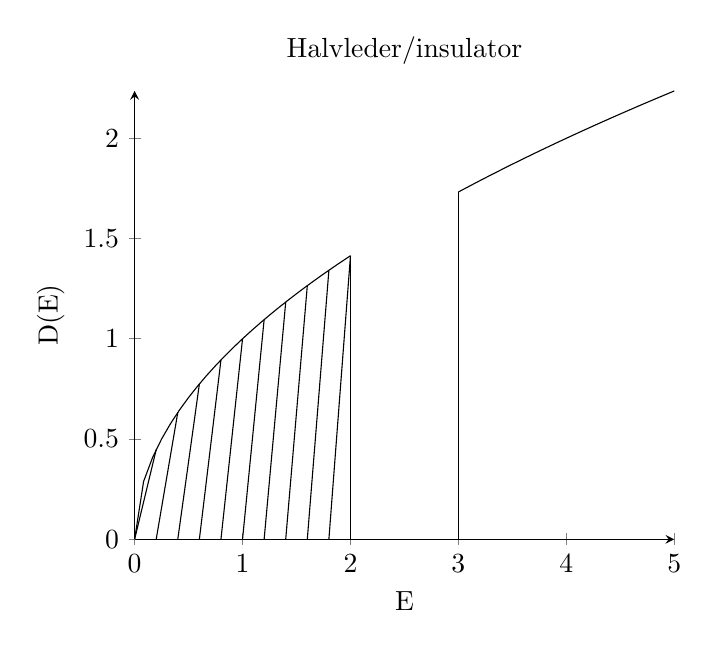
\begin{tikzpicture}
  \begin{axis}[
    axis lines = left,
    title = Halvleder/insulator,
    xlabel = E,
    ylabel = D(E),
  ]
  \addplot[domain=0:2,color=black]{sqrt(x)};
  \addplot[mark=none, black] coordinates {(0.2,0.4472135955) (0,0)};
  \addplot[mark=none, black] coordinates {(0.4,0.63245553203) (0.2,0)};
  \addplot[mark=none, black] coordinates {(0.6,0.77459666924) (0.4,0)};
  \addplot[mark=none, black] coordinates {(0.8, 0.894427191) (0.6,0)};
  \addplot[mark=none, black] coordinates {(1, 1) (0.8,0)};
  \addplot[mark=none, black] coordinates {(1.2, 1.09544511501) (1,0)};
  \addplot[mark=none, black] coordinates {(1.4, 1.18321595662) (1.2,0)};
  \addplot[mark=none, black] coordinates {(1.6, 1.26491106407) (1.4,0)};
  \addplot[mark=none, black] coordinates {(1.8, 1.3416407865) (1.6,0)};
  \addplot[mark=none, black] coordinates {(2, 1.41421356237) (1.8,0)};
  \addplot[mark=none, black] coordinates {(2, 1.41421356237) (2,0)};
  \addplot[domain=2:3,color=black]{0};
  \addplot[mark=none, black] coordinates {(3,0) (3,1.73205080757)};
  \addplot[domain=3:5,color=black]{sqrt(x)};
  \end{axis}
\end{tikzpicture}

% HER Videre har vi... (legg til mer her Sebastian)
Noter at det kjemiske potensialet $\mu$ er i midten av båndgapet.
\dots

\subsection{Hull}
Et hull er en ledig orbital ("tilstand") i et ellers fylt bånd. Det oppfører seg som en partikkel med motsatt ladning til elektronene i båndene. Den effektive massen til et slikt hull vil også være motsatt. Altså $m^{*}_h = -m_e^{*}$.

Fra før visste vi at effektiv masse $m^* \defeq \left(\hbar^2 \frac{d^2 E}{dk^2}\right)^{-1}$
Har vi huller i båndene våre kan elektronene bevege seg i motsatt retning i forhold til det man hadde forventet når man legger til et potnesial. Altås får man da en slags negativ effektive masse på elektronene, mens hullene får en positiv masse.

\subsubsection{Båndstrukturen til GaAs og silikon}
\begin{tikzpicture}
  \begin{axis}[
    axis lines = left,
    title = Båndstukturen til GaAs,
    xlabel = k,
    ylabel = E,
  ]
  \addplot[domain=-5:5,color=black]{cosh(x / 2) + 3};
  \addplot[mark=none, black, dotted] coordinates {(-5,0) (5, 0)};
  \addplot[mark=none, red, dotted] coordinates {(-5,1.5) (5, 1.5)};
  \addplot[domain=-5:5,color=black]{-cosh(x / 2) - 4};
  \end{axis}
\end{tikzpicture}
\hskip 5pt
\begin{tikzpicture}
  \begin{axis}[
    axis lines = left,
    title = Båndstukturen til Silicon,
    xlabel = k,
    ylabel = E,
  ]
  \addplot[domain=-10:10,color=black]{cos(x / (2 * pi) * 360 / 2.25) * 10 + 20};
  \addplot[mark=none, black, dotted, thick] coordinates {(-10,0) (10, 0)};
  \addplot[mark=none, red, thick, dotted] coordinates {(-10,5) (10, 5)};
  \addplot[domain=-6:6,color=black]{-cosh(x / 3) * 8 - 10};
  \end{axis}
\end{tikzpicture}

Her blir båndet under valensbåndet og båndet over er ledningsbåndet. I tillegg representerer linjen i mitten energien $E = 0$, og den røde linjen er det kjemiske potensialet $\mu$. Vi ser også at fermi-fordelingen faller av fort. Altså er de mest mest interessante elektronene plassert på steder hvor vi har høyest aksellerasjon. På grafen til venstre har vi et direkte båndgap. Får å hoppe over må vi ha et foton med $E = E_g$ for å eksitere et elektron fra valensbåndet til ledningsbåndet. Energien her er neglisjerbar og er en vertikal prosess hvor elektroner hopper opp i energi med samme k.

I tillegg har vi her et \underline{Indirekte} båndgap på høyresiden fordi elektroner må endre k mer. Altså er "fononassistens" et krav og da er det mindre sannsynlig. Her til høyre får vi et båndgap på $E_g = 1.11 eV$. For å eksitere elektronene trenger de et foton med $E = E_g$, i tillegg ødelegger eller skaper man et fonon med $\Delta k$ krystall momentum for å få til eksitasjonen.


For solpaneler vil man ha et direkte båndgap som for eksempel GaAs fordi det bir bedre ytelse men der dyrere. Altså bruker satelitter GaAs mens hus bruker Si.

Videre vil jeg definere "Radierende Rekombinasjon":
\begin{itemize}
  \item Fotoner er emittert når elektroner går fra ledningsbåndet til valensbåndet.
  \item LED (light emitting diodes) (lys emitterende dioder)
\end{itemize}

Hvis vi ser på et foton som har lik energi som båndgapet har vi:
\begin{align*}
  \hbar \omega_{optisk} = E_g \\
  \omega \propto \frac{E_g}{\hbar} \propto 10^{14} s^{-1} \\
  k_{optisk} = \frac{\omega_{optisk}}{c} \propto 10^6 m^{-1}
\end{align*}
Sammenlign med $g_1 = \frac{2 \pi}{a} \propto 10^{10} m^{-1}$.

Altså ser vi at endringen man ville hatt i momentum ikke er i nærheten av nok til å komme seg ut av B.S-en. Altså er prosessen her en vertikal prosess til en veldig god approksimasjon. 

\subsubsection{Å bruke absorbsjon til å forstå halvledere}
Vi kan bruke lys til å forstå halvledere. La oss se på hvor mye lys som er absorbert i forhold til energi:
\begin{tikzpicture}
  \centering
  \begin{axis}[
    axis lines = left,
    title = Lys absorbsjonn,
    xlabel = k,
    ylabel = E,
    width = 10cm,
    height = 7cm
  ]
  \addplot[domain=5:10, red]{3 / (1 + e^(-(x - 7.5)*1.5))};
  \addplot[domain=5:10, blue]{3 / (1 + e^(-(x - 8.5)*5))};
  \addplot[mark=none, black, dotted, thick] coordinates {(0,0) (0, 5)};
  \end{axis}
\end{tikzpicture}


Her er de to fargene direkte versus inderekte absorbsjon. Altså ser vi at de to tilfellene gir forskjellige grafer.
\begin{equation*}
  I(\lambda) = I_0(\lambda) e^{-\mu (\lambda) s}
\end{equation*}



% IVars notater
% Forelesning en eller annen gang



% Forelesning 15.04.2024
\subsection{Inneboende/Rene halvledere}
\subsection{Dopede/Urene halvledere}
Som vi har utledet i forrige delkappitel hadde vi at:
\begin{align*}
  n &= \frac{1}{V} \int_{E_g}^{\infty} D_c(E) f_c(E, T)dE = \underbrace{\frac{1}{\sqrt{2}} \left( \frac{m_e^{*} k_B T}{\pi \hbar^2}\right)^{\frac{3}{2}} e^{-\frac{(E_g - \mu)}{k_B T}} }_{\propto 10^{25} m^{-3}\text{ for } T \approx T_{\text{romtemp}}} \\
  p &=\frac{1}{V} \int_{-\infty}^0 D_v(E) (1-f_e) dE = \frac{1}{\sqrt{2}} \left( \frac{m_h^{*} k_B T}{\pi \hbar^2}\right)^{\frac{3}{2}} e^{-\frac{\mu}{k_B T}}\\
  \Rightarrow np &= 4 \left(\frac{k_B T}{2 \pi \hbar^2}\right)^3 (m_e^{*} m_h^{*})^{\frac{3}{2}} e^{-\frac{E_g}{k_B T}}
\end{align*}
Altså har vi ingen $\mu$-avhengighet. Ved inneboende halvledere har vi at $n=p$ (noter at np = konstant), som gir oss (ved å løse likningene over for $\mu$):
\begin{equation*}
  \mu = \frac{E_g}{2} + \frac{3}{4} k_B T \ln{\left(\frac{m_h^{*}}{m_e^{*}}  \right)}
\end{equation*}
Nå har vi da at dopede halvledere deles inn i to grupper. N og P-type.
\begin{itemize}
  \item N-Type:
  \begin{itemize}
    \item Det er donor-urenheter i dem. Altså atomer som vil donere vekk elektroner til omgivelsene.
    \item Ved å bruke Si og Ge så brukes oftest gruppe 5 elementer for å dope. Hovedbæreren i halvlederene er elektroner
  \end{itemize}
  \item P-Type: 
  \begin{itemize}
    \item Det er motager-urenheter. Altså atomer som gjerne tar imot elektroner fra omgivelsene.
    \item Igjen er det Si og Ge som brukes, men for å dope her bruker mann som oftest gruppe 3 elementer. Hovedbæreren i disse halvlederene er hull.
  \end{itemize}
\end{itemize}
Typiske tall her er da at man har mellom  0.0000001\% - 0.001\% med urenheter i et stoff. Å notere seg her er at Si har $5 * 10^{28}$ atomer per $m^3$, og en inneboende Ladningsbærerkonsentrasjon på $\approx 10^{16}$ per $m^3$ ved romtemperatur. Oppsummert kan vi da se at vi bruker elementer fra gruppe 4 som Si og Ge og doper dem med donorer eller motagere av elektroner fra gruppe 3 og 5. Slike små addisjoner av stoffer kan faktisk øke konduktiviteten til et stoff med hele 10 000x!

Denne dopingen gir nye tilstander i båndgapet og endrer det kjemiske potensialet. Disse ligger mellom ledningsbåndet og valensbåndet og for en n-type halvleder ligger den over, mens for en p-type halvleder ligger den under. Da flyttes det kjemiske potensialet fra halvveis til mellom disse donortilstandene og ledningsbåndet for n-type halvledere mens for p-type halvledere ligger de da nede mellom donortilstandene og  valensbåndet.

Ved en lav temperatur har man for donorer at $\mu$ må være mellom donortilstandene og lednignsbåndet. Ved en høyere temperatur vil alle donorelektroner gå i ledningsbåndet mens $\mu$ vil bevege seg mot $\frac{E_g}{2}$ fordi man da må ta elektroner fra valensbåndet for å eksitere dem til ledningsbåndet.
\section{Kapittel IX: Nanoforskning}
Hvorfor er  folk så interesserte i nanoforskning? Vel. Vi kan begynne med å se på endelige faste stoffer (nano-strukturer). Når vi er i disse små skaalaene får vi kvanteinnesperring, endring av bulken, og vi har et stort overflateareal med reaksjoner.

Så langt i kurset har vi snakket om periodiske grensebetingelser. Vi har gjort dette for å fjerne alle overflateeffektene. Altså er vi uavhengige av hvor vi er på overflaten ved at vi har et potensial $u(x,y,z)=u(x+L,y+L,z+L)$. På grunn av disse periodiske grensebetingelsene får vi at momentumet til partikler i systemet er kvantiserte: $k = \frac{2 \pi}{a N} n$. Vi har også da at N atomer vil gi N normalmoder av vibrasjon. For lange men endelige kjeder vil tilstandstettheten være høy. Når vi har en film av tykkelse $d \propto \lambda$, vil vi ha kvanteeffekter gjennom dimensjonen til denne tykkelsen. Altså kan man få fripartikkelø tilstander langs den lengden som er veldig lang $k = \frac{2\pi}{\lambda}$, men kvantiserte tilstander langs den tynne lengden.

Områder man kan bruke dette er hvis man har en halvleder og et vakuum. Hvis man setter en tynn film over halvlederen, vil vi få en slags brønn i potensialet mellom halvlederen og vakuumet. Da kan vi gjøre en Ansatz: $\psi_{tot}(r) = \psi(z) \psi_{side}(x,y)$ hvor: $\psi(z) = Ae^{ik_z z}+Be^{-ik_z z}$. Hvis man da har en uendelig brønn, må bølgefunksjonen være null ved overgangen mellom disse tre stoffene. Da får vi det som kalles for en De-Broglie-betingelse: $2d = n\lambda \Rightarrow 2k_z d = 2\pi n$, som gir oss at:
\begin{equation*}
  E_n = \frac{\hbar^2 k_z^2}{2m} = \frac{n^2 \pi^2 \hbar^2}{2m d^2}
\end{equation*}

For en endelig brønn kan man vise at: $2k_z d + \Phi_i + \Phi_v = 2\pi n$.

\subsection{Kvantekorall}
En kvantekorall har en diameter på $\approx 70 Å$. Man før frie elektroner på overfaltten denne ligger på. Den er også bygget opp av cirka 50 jernatomer på en kobberoverflatefilm. Se bildet for hvordan de ser ut:
\begin{figure}[h]
  \centering
  \caption{Kvantekorallen}
  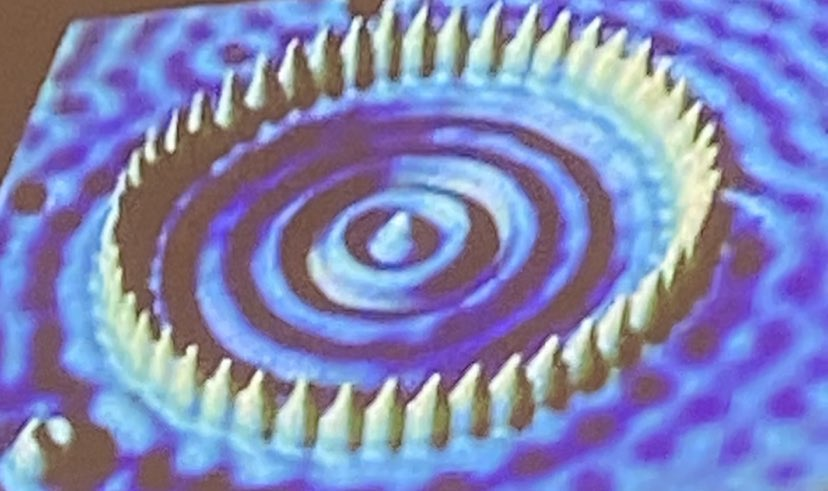
\includegraphics[scale=0.4]{bilder/kvantekorallen.jpg}
  \label{fig:kvantekorallen}
\end{figure}

Den letteste måten å modellere denne er ved å velge et potensial som er uendelig utenfor korallen og 0 innenfor. Altså blir dette en sfærisk uendelig brønn. Med dette potensialet får vi løsninger i formen til bessel-funksjonene: $\\psi_x(R) = AJ_m(kr) + \underbrace{BY_m(kr)}_{=0 \text{ fordi $Y_m$ divergerer når $r\rightarrow 0$}}$, med betingelsen $J_m(ka)$ og $\varepsilon = \frac{\hbar^2 \alpha*2}{2ma^2}$
\subsection{Halvleder-nanopartikler / Kvantepunkter ($r \le 100nm$)}
For å lage et elektron-hull par må du ha like mye energi som båndgapet i halvederen. I en halvleder nano-krystall vil vi få:
\begin{equation}
  E^{\text{nano}}_{\text{min}} = E_{\text{gap}} + \underbrace{ \frac{\hbar^2 \pi^2}{2 \mu r^2}}_{\substack{\text{Kvanteinnespering av elektronet og hullet} \\ \text{ som begge er lokalisert mer enn i bulken.}}} - \underbrace{\frac{1.8 e^2}{4 \pi \varepsilon_0 r}}_{\text{Coloumb-vekselsvirkning mellom hullet og elektronet}}
\end{equation}
Hvor her $\mu$ er den reduserte massen til elektronet og hullets effektive masser. Noter her også at det første leddet har med dreieimpulsen til dette paret å gjøre og avhenger av $1/r^2$. Disse kvantepunktene vil også endre på båndgapet. Jo mindre de er, jo større er båndgapet. I tillegg endrer jo da fargen til disse kvantepunktene seg til å bli blåere ved en høyere energi. Her kan man se kvanteeffektene i et bilde som viser slike kvantepunkter i et stoff preparert i ulike størrelser:
\begin{figure}[h]
  \centering
  \caption{Kvantepunktstoff}
  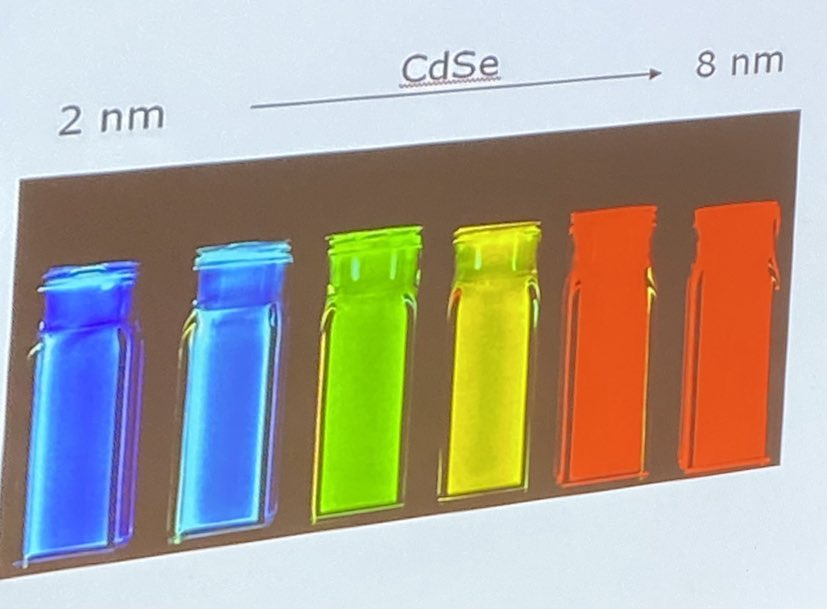
\includegraphics[scale=0.4]{bilder/kvantepunktstoff.jpg}
  \label{fig:kvantepunktstoff}
\end{figure}


\newpage
\printbibliography

\end{document}